% ACM MHV'27 one-page extended abstract. Build: latexmk -pdf abstract.tex
% Sources (all in results/experiment26/mhv/): render_comparison.ps1 + make_results_figure.py
% (Fig. 1: new renders, light-video frames not used in the paper), codec_partition_stats.py +
% stats.json (Table 1).
\documentclass[sigconf]{acmart}
\usepackage{booktabs}
% Uniform 0.6in margins (set via \newgeometry after \begin{document}, since acmart fixes the
% page layout at load time); the MHV abstract format is not strict.

\settopmatter{printacmref=false, printccs=false, printfolios=false}
\setcopyright{none}
\renewcommand\footnotetextcopyrightpermission[1]{}
\acmConference[MHV '27]{ACM Mile-High Video Conference}{2027}{Denver, CO, USA}
\citestyle{acmauthoryear}
\setlength{\textfloatsep}{8pt plus 2pt minus 2pt}
\setlength{\floatsep}{6pt plus 2pt minus 2pt}
\raggedbottom
\captionsetup{skip=3pt}

\begin{document}
\newgeometry{margin=0.6in, headheight=10pt, headsep=10pt, footskip=0pt}

\title{Importance Sampling Video Light Sources with Codec Partitions}

\author{Jose Aguerre}
\affiliation{\institution{Evercast}\country{USA}}
\email{jose.aguerre@evercast.com}

\begin{teaserfigure}
  \centering
  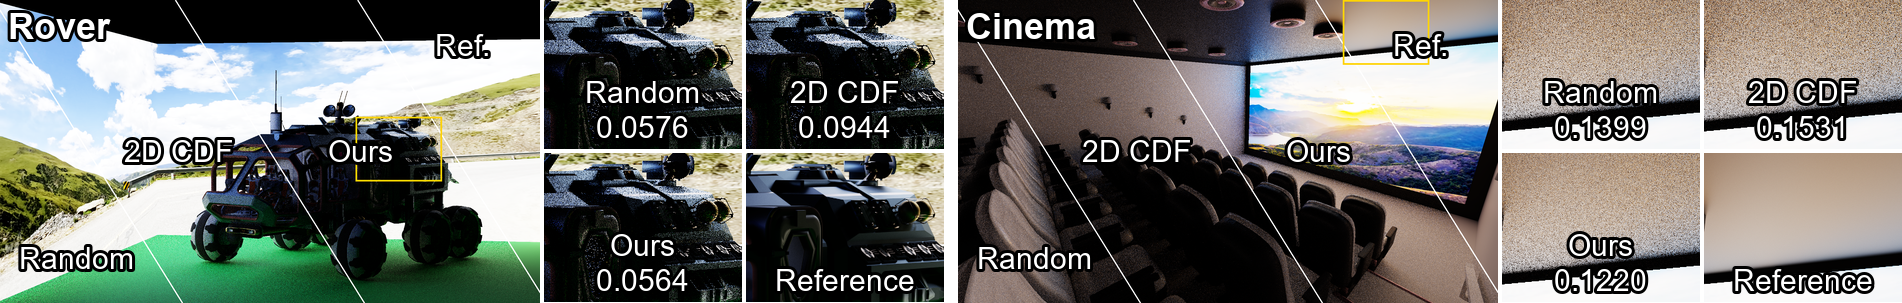
\includegraphics[width=\textwidth]{results_strip.png}
  \caption{Random, dense 2D CDF and codec sampler (Ours) at 33\,ms against a converged reference;
  closeups show RMSE.}
  \label{fig:results}
\end{teaserfigure}

\maketitle

\section{Introduction}

We introduce an efficient technique for importance sampling emissive textures used in
video-driven lighting for virtual production, AR/VR and visual effects, where an HDR video shown
on an LED wall, a virtual screen or an environment map must illuminate synthetic geometry in real
time. Monte Carlo renderers importance sample such a source in proportion to its radiance, but
dense structures such as a 2D CDF must be rebuilt for every frame, at a high cost in time and
memory bandwidth.

Compressed video formats such as VP9, HEVC and AV1 already represent each frame through coding
trees refined where the signal
varies~\cite{sullivan2012hevc,mukherjee2013vp9,han2021av1}, and the transform
coefficients~\cite{ahmed1974dct} of each block encode its mean (DC) and its low-frequency
variation (AC). We repurpose
this hierarchy as a sampling structure without additional spatial analysis: the mean luminance
of each block turns the coding tree into an alias table that draws light samples in constant
time, removing the dense CDF, lowering memory bandwidth and enabling real-time lighting from
video. It extends a preliminary hierarchical-CDF version~\cite{aguerre2026codec}.

\section{Method and Results}

We encode each light video with libvpx (VP9 Profile~2, 10-bit) at a speed setting that uses the
variance-based partitioning rule, and export from the decoder each frame's superblock partition
($64{\times}64$ down to $8{\times}8$ pixels) and block coefficients. Each coded block becomes a
leaf $i$ with area $A_i$, mean luminance $\bar L_i$ taken from its DC term in linear light, and
flux weight $w_i = A_i \bar L_i$. A Walker/Vose alias table over these weights is built in
$O(n)$. A sample picks a leaf in $O(1)$ and a uniform point inside it, with density
$\bar L_i/\sum_j w_j$, and an index map with one entry per $8{\times}8$ cell returns the same
density for multiple importance sampling. At 16 bytes per leaf, the structure takes
0.12--0.8\,MB and is built in under 1\,ms per frame, versus about 10\,ms (Full HD) and 33\,MB (4K)
for a dense CDF.

In a GPU path tracer calibrated to 33\,ms per frame (RTX 4080 SUPER), the
saved time buys more light samples, and the codec sampler has the lowest RMSE against a converged
reference on Rover, Cinema and Fireplace Room, 10--40\% below the dense CDF
(Fig.~\ref{fig:results} shows the first two). We also score densities $q$ over every fifth frame
by the relative variance of a one-sample flux estimate, $\chi^2 = \sum_x p^*(x)^2/q(x) - 1$ with
$p^* = L/\sum_x L$ (Table~\ref{tab:chi2}). The coding tree lowers $\chi^2$ by 9--87$\times$
relative to uniform (Random) sampling and by 2.5--7.1$\times$ relative to $64{\times}64$
superblock means.

\begin{table}[t]
\caption{$\chi^2$ per frame (SB: superblock means; G8: $8{\times}8$ grid).}
\label{tab:chi2}
\footnotesize
\setlength{\tabcolsep}{4pt}
\begin{tabular}{l c r r r r r r}
\toprule
Sequence & Res. & Leaves & Uniform & SB & DC & +AC & G8 \\
\midrule
Rover     & 1080p & 10.7k & 0.636 & 0.186 & 0.071 & 0.045 & \textbf{0.044} \\
Cinema    & 1080p & 7.4k  & 0.958 & 0.087 & 0.035 & 0.018 & \textbf{0.011} \\
Fireplace & 4K    & 50.1k & 8.153 & 0.664 & 0.094 & \textbf{0.037} & 0.070 \\
\bottomrule
\end{tabular}
\end{table}

\section{Discussion}

Other libvpx speed settings use rate-distortion search or reuse partitions, so their trees follow
coding cost and motion. HEVC~\cite{sullivan2012hevc}, AV1~\cite{han2021av1} and VVC~\cite{bross2021vvc} partitions, including binary,
ternary and T-shaped splits, also yield rectangles the alias table handles unchanged; where a
tree is not variance-driven, Parseval's theorem gives a block's variance from its AC energy, so
leaves can be split or merged in the compressed domain.

The DC coefficient of a predicted block is the mean of its residual, so in inter frames it is a
difference to the motion-compensated reference. As interpolation filters have unit DC gain, a DC
image of the reference frame can track block means~\cite{yeo1995rapid}, with a drift that resets
at keyframes; intra blocks use the reconstructed block. For HDR, the mean of PQ or HLG code values
underestimates the linear mean of textured blocks. These errors add variance but no bias, since
sampling and weighting share one density.

The first AC coefficients describe how brightness tilts across a block; a sloped density built
from them inside each leaf keeps closed-form sampling and lowers $\chi^2$ by a further 37--61\%
(Table~\ref{tab:chi2}), though it is untested in the renderer. Exposing these terms as decoder
side data, which hardware decoders lack, would let a renderer sample an LED-wall feed directly.

\bibliographystyle{ACM-Reference-Format}
\bibliography{refs}

\end{document}
